\documentclass[12pt,t]{beamer}
% \documentclass[t]{beamer}
\usepackage[utf8]{inputenc}
\usepackage[catalan]{babel}
\usepackage{verbatim}
\usepackage{hyperref}
\usepackage{amsfonts,amssymb,amsmath,amsthm, wasysym}
\usepackage{listings}
\usepackage[T1]{fontenc}        
\usepackage{pgf}
\usepackage{epsdice}
\usepackage{pgfpages}
\usepackage{tikz}
%\usetikzlibrary{arrows,shapes,plotmarks,backgrounds,trees,positioning}
%\usetikzlibrary{decorations.pathmorphing,calc,snakes}
%\usepackage{marvosym}
%
\usetheme[hideothersubsections,left]{Marburg}
\usecolortheme{sidebartab}
\useinnertheme[shadow]{rounded}
% \useoutertheme[footline=empty,subsection=true,compress]{infolines}
% \useoutertheme[footline=empty,subsection=true,compress]{miniframes}
% \usefonttheme{serif}

\setbeamertemplate{caption}[numbered]
\setbeamertemplate{navigation symbols}{}


\newcommand{\red}[1]{\textcolor{red}{#1}}
\newcommand{\green}[1]{\textcolor{green}{#1}}
\newcommand{\blue}[1]{\textcolor{blue}{#1}}
\newcommand{\gray}[1]{\textcolor{gray}{#1}}
\renewcommand{\emph}[1]{{\color{red}#1}}

\setbeamertemplate{frametitle}
{\begin{centering}
\medskip
\color{blue}
\textbf{\insertframetitle}
\medskip
\end{centering}
}
\usecolortheme{rose}
\usecolortheme{dolphin}
\mode<presentation>


\newcommand{\CC}{\mathbb{C}}
\newcommand{\RR}{\mathbb{R}}
\newcommand{\ZZ}{\mathbb{Z}}
\newcommand{\NN}{\mathbb{N}}
\newcommand{\KK}{\mathbb{K}}
\newcommand{\MM}{\mathcal{M}}
%\newcommand{\dbinom}{\displaystyle\binom}

\newcommand{\limn}{{\displaystyle \lim_{n\to\infty}}}
\renewcommand{\leq}{\leqslant}
\renewcommand{\geq}{\geqslant}
\def\tendeix{{\displaystyle\mathop{\longrightarrow}_{\scriptscriptstyle
n\to\infty}}}

\newcommand{\matriu}[1]{\left(\begin{matrix} #1 \end{matrix}\right)}

% \newcommand{\qed}{\hbox{}\nobreak\hfill\vrule width 1.4mm height 1.4mm depth 0mm
%     \par \goodbreak \smallskip}
%
% %
\theoremstyle{plain}
\newtheorem{teorema}{Teorema}
\newtheorem{prop}{Proposició}
\newtheorem{cor}{Coro\l.lari}
\theoremstyle{definition}
\newtheorem{exemple}{Exemple}
\newtheorem{defin}{Definició}
\newtheorem{obs}{Observació}

\newcounter{seccions}
\newcommand{\seccio}[1]{\addtocounter{seccions}{1}
\medskip\par\noindent\textbf{\theseccions.
#1}\smallskip\par }

\newcommand{\EM}{\Omega}
\newcommand{\PP}{\mathcal{P}}

\title[\red{Matemàtiques III}]{}
\author[]{}
\date{}



\begin{document}
\beamertemplatedotitem

\lstset{backgroundcolor=\color{green!50}}
\lstset{breaklines=true}
\lstset{basicstyle=\ttfamily}


\section{Estimació puntual}

\begin{frame}
\vfill
\begin{center}
\gray{\LARGE Estimació puntual}
\end{center}
\vfill
\end{frame}






\subsection{Definicions bàsiques}


\begin{frame}
\frametitle{Estadística inferencial}

El problema típic de l'\emph{estadística inferencial} és:

\begin{itemize}

\item Volem conèixer el valor  d'una característica en el global d'una població
\medskip

\item No podem mesurar aquesta característica en tots els individus de la població
\medskip

\item Extraiem una mostra aleatòria de la població, mesuram la característica en els individus d'aquesta mostra i \emph{inferim} el valor de la característica en el global de la població

\begin{itemize}
\item Com ho hem de fer?
\item Com ha de ser la mostra?
\item Quina informació podem inferir de veritat?
\end{itemize}
\end{itemize}
\end{frame}



\begin{frame}
\frametitle{Exemples}

\begin{center}
\hspace*{-0.5cm}

\includegraphics[width=1.1\linewidth]{plagiUIB1.jpg}\pause\bigskip

\hspace*{-0.5cm}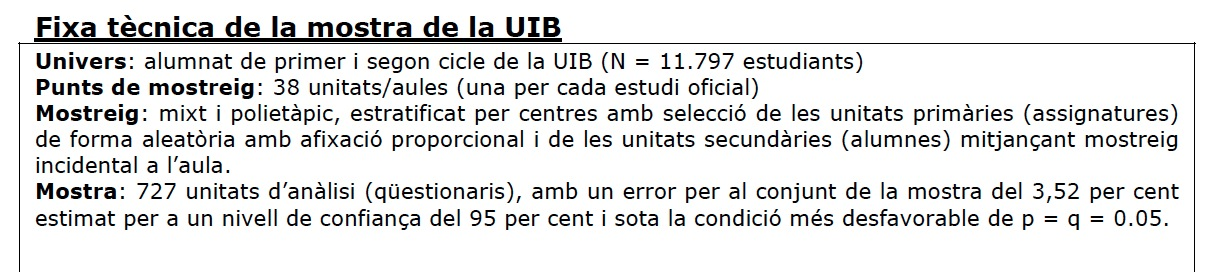
\includegraphics[width=1.1\linewidth]{plagiUIB2.jpg}
\end{center}
\end{frame}


%
%\begin{frame}
%\frametitle{Exemples}
%\vspace*{-0.5cm}
%
%\begin{center}
%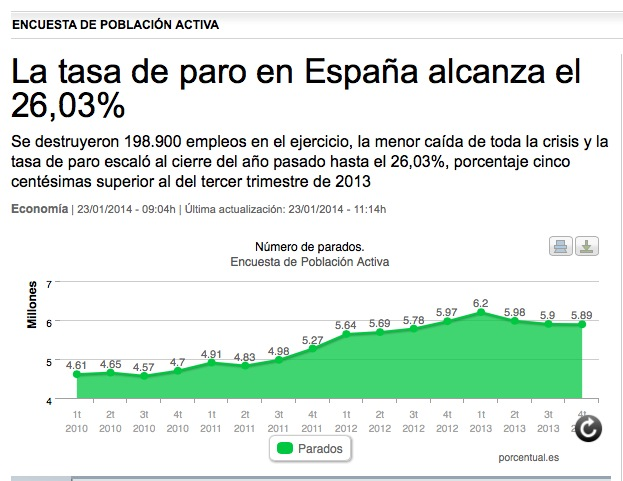
\includegraphics[width=\linewidth]{paro.jpg}
%\end{center}
%\end{frame}

\begin{frame}
\frametitle{Exemples}


\begin{center}

\includegraphics[width=\linewidth]{vacuna1.jpg}\medskip


\includegraphics[width=\linewidth]{vacuna2.jpg}
\end{center}


{\footnotesize \url{http://www.scielosp.org/pdf/rpsp/v8n6/3956.pdf}}
\end{frame}

\begin{frame}
\frametitle{Definicions bàsiques}

\emph{Mostra aleatòria simple (m.a.s.) de mida $n$:} D'una població de $N$ individus, repetim $n$ vegades el procés d'escollir equiprobablement un individu; \textit{els individus triats es poden repetir}
\bigskip

\blue{Exemple:} Escollim a l'atzar $n$ estudiants de la UIB (amb reposició) per midar-los l'alçada
\bigskip

D'aquesta manera, totes les mostres possibles de $n$ individus (possiblement repetits: \emph{multiconjunts}) tenen la mateixa probabilitat
\bigskip

\emph{\bf Llegiu-vos aviat la lliçó 1 de R sobre Mostreig}
\end{frame}


\begin{frame}
\frametitle{Definicions bàsiques}

\emph{Estadístic} (\emph{Estimador puntual}): Una funció que aplicada a una mostra ens permet \emph{estimar} un valor que vulguem saber de tota la població
\bigskip

\blue{Exemple:} La mitjana de les alçades d'una mostra d'estudiants de la UIB ens permet estimar la mitjana de les alçades de tots els estudiants de la UIB
\bigskip

\end{frame}

\begin{frame}
\frametitle{Formalment}

Una \emph{m.a.s.\ de mida $n$} (d'una v.a.\ $X$) és
\begin{itemize}
\item  un conjunt de $n$ còpies \blue{independents} de $X$, o

\item un conjunt de $n$ variables aleatòries  \blue{independents} $X_1,\ldots,X_n$, totes amb la distribució de  $X$
\end{itemize}
\medskip


\blue{Exemple:} Sigui $X$ la v.a.\ ``triam un estudiant de la UIB i li mesuram l'alçada''. Una m.a.s.\ de $X$ de mida $n$ seran $n$ còpies independents $X_1,\ldots,X_n$ d'aquesta $X$.
\bigskip


Una \emph{realització} d'una m.a.s.\ són els $n$ valors $x_1,\ldots,x_n$ que prenen les v.a.\ $X_1,\ldots,X_n$

\end{frame}


\begin{frame}
\frametitle{Formalment}

Un  \emph{estadístic} $T$ és una funció aplicada a la mostra $X_1,\ldots,X_n$:
$$
T=f(X_1,\ldots,X_n)
$$
Aquest estadístic s'aplica a les realitzacions de la mostra
\medskip

\blue{Exemple:} La \emph{mitjana mostral} de una m.a.s.\ $X_1,\ldots,X_n$ de mida $n$ és 
$$
\overline{X}:=\frac{X_1+\cdots+X_n}{n}
$$
Estima $E(X)$
\medskip

\blue{Exemple:} La mitjana mostral de les alçades d'una  realització d'una m.a.s.\ d'alçades d'estudiants estima  l'alçada mitjana d'un estudiant de la UIB




\end{frame}


\begin{frame}
\frametitle{Formalment}

Un  \emph{estadístic} $T$ és una funció aplicada a la mostra $X_1,\ldots,X_n$
$$
T=f(X_1,\ldots,X_n)
$$
\medskip

Per tant, un estadístic és una (nova) variable aleatòria, amb distribució, esperança, etc.
\medskip

La \emph{distribució mostral} de $T$ és la distribució d'aquesta variable aleatòria
\medskip

Del coneixement d'aquesta distribució mostral, podrem estimar propietats de $X$ a partir de les  d'una mostra
\medskip

\emph{Error estàndard de $T$}: desviació típica de $T$


\end{frame}



\begin{frame}
\frametitle{Conveni}

\emph{\bf ELS ESTADÍSTICS, EN MAJÚSCULES; les realitzacions, en minúscules}
\medskip

\blue{Exemple:} 
\begin{itemize}
\item $X_1,\ldots,X_n$ una m.a.s.\ i 
$$
\overline{X}:=\frac{X_1+\cdots+X_n}{n}
$$
la mitjana mostral\medskip


\item $x_1,\ldots,x_n$ una realització d'aquesta m.a.s.\ i 
$$
\overline{x}:=\frac{x_1+\cdots+x_n}{n}
$$
la mitjana (mostral) d'aquesta realització
\end{itemize}

\end{frame}




\begin{frame}
\frametitle{La vida real}

A la vida real, les mostres aleatòries se solen prendre sense reposició (sense repeticions).
No són mostres aleatòries simples. Però:
\begin{itemize}
\item Si $N$ és molt més gran que $n$,  els resultats per a m.a.s.\ valen (aproximadament) en aquest cas, perquè les repeticions són improbables i les variables aleatòries que formen la mostra són gairebé independents
\smallskip

 Farem l'abús de llenguatge de dir que en aquest cas també tenim una m.a.s.
\medskip

\item Si $n$ és relativament gran, sovint es poden donar versions corregides dels estadístics
\end{itemize}

\end{frame}


\begin{frame}
\frametitle{La vida real}

\blue{Exemple:} La UIB té uns 12000 estudiants

\begin{center}
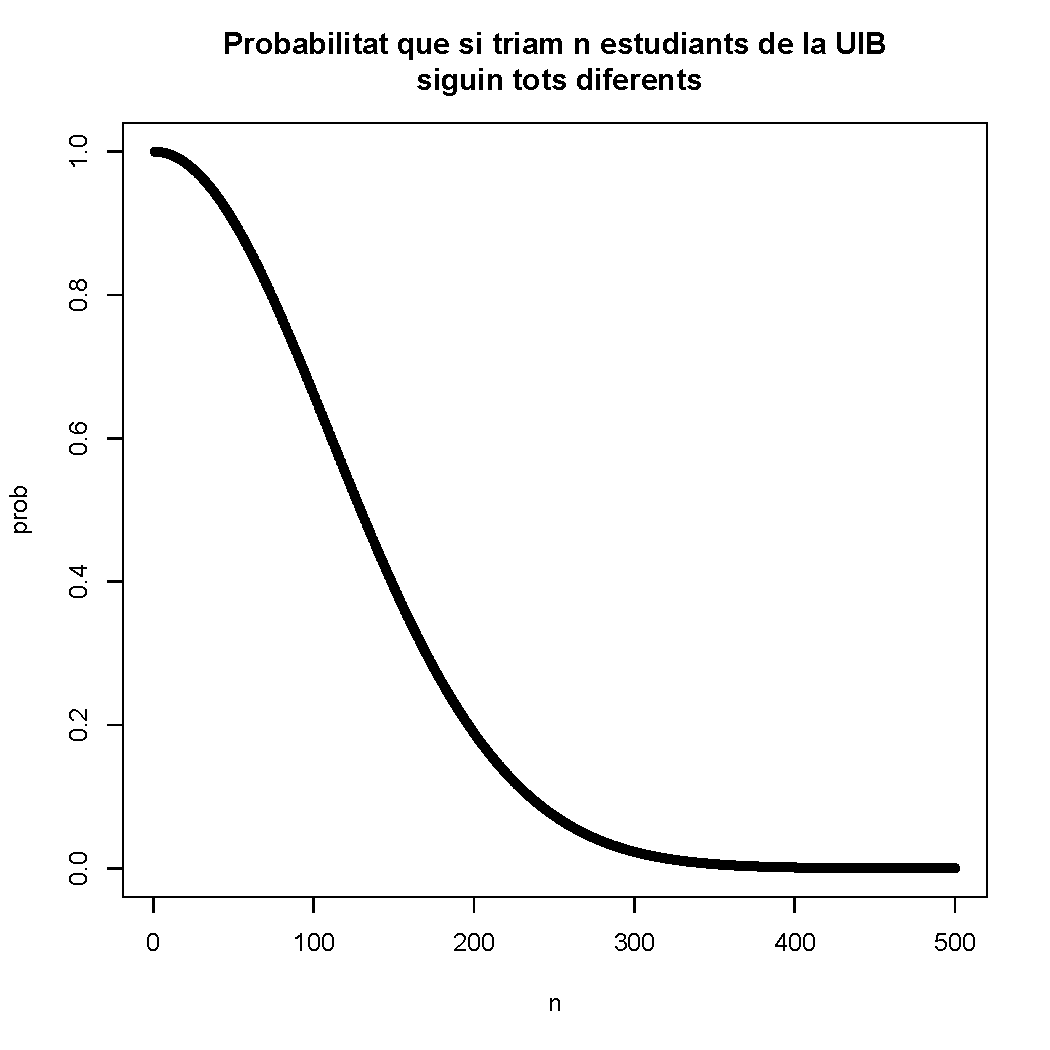
\includegraphics[width=0.8\linewidth]{UIB.pdf}
\end{center}

\end{frame}


%%Concurs1
%La UIB té uns 16000 estudiants. 
%
%a) Quina és la probabilitat que si en triam n a l'atzar, un rere l'altre i amb reposició, siguin tots diferents?
%b) Definiu una funció de R que, aplicada a n, doni aquesta probabilitat
%c) Calculau la llista $(f(n))_{n=2,150}$ (per aplicar una funció a una llista, si directament no funciona, podeu emprar sapply(llista, funció)). Quin és el nombre màxim d'estudiants que podem triar de manera que la probabilitat que siguin tots diferents sigui com a mínim del 95\%?
%d) La funció $f$, és aproximadament lineal, polinòmica o exponencial (o cap de les tres coses) en $n$? En cas afirmatiu, trobau la funció que l'aproxima, i confirmau amb un gràfic aquesta aproximació.



\subsection{Mitjana mostral}
\begin{frame}
\frametitle{Mitjana mostral}

Sigui $X_1,\ldots, X_n$ una m.a.s.\ de mida $n$ d'una v.a.\ $X$ d'esperança $\mu_X$ i desviació típica $\sigma_X$
\medskip

La \emph{mitjana mostral} és
$$
\overline{X}=\frac{X_1+\cdots+X_n}{n}
$$

\begin{teorema}
En aquestes condicions
$$
E(\overline{X})=\mu_X,\quad \sigma_{\overline{X}}=\frac{\sigma_X}{\sqrt{n}}
$$
\end{teorema}

 $\sigma_{\overline{X}}$ és l'\emph{error estàndard} de $\overline{X}$



\end{frame}

\begin{frame}
\frametitle{Mitjana mostral}

$$
\overline{X}=\frac{X_1+\cdots+X_n}{n}
$$
\begin{itemize}
\item És un estimador puntual de $\mu_X$
\medskip

\item \emph{$E(\overline{X})=\mu_X$}
\begin{itemize}
\item El valor esperat de $\overline{X}$ és $\mu_X$
\medskip

\item Si prenem moltes vegades una m.a.s.\ i en calculam la mitjana mostral, el valor mitjà d'aquestes mitjanes tendeix molt probablement a ser $\mu_X$
\end{itemize}
\bigskip

\item \emph{$\sigma_{\overline{X}}= \sigma_X/\sqrt{n}$}: la variabilitat dels resultats de $\overline{X}$ tendeix a 0 quan prenem mostres grans
\end{itemize}

\end{frame}

\begin{frame}[fragile]
\frametitle{Mitjana mostral}
\vspace*{-2ex}

{\small
\begin{verbatim}
> # tests.txt=notes dels tests de BL i BQ
> tests=scan("tests.txt")
Read 185 items
> mean(tests)
[1] 55.43243
> set.seed(100)
> mitjanes=replicate(10^4,
    mean(sample(tests,40,rep=TRUE)))
> mean(mitjanes)
[1] 55.45814
> #sd, per fer via
> c(sd(tests)/sqrt(40),sd(mitjanes))
[1] 3.390031 3.420459
\end{verbatim}
}

\end{frame}







\begin{frame}
\frametitle{Exemple}

S'ha pres una m.a.s.\ de 10 estudiants de la UIB, i les seves alçades han estat
$$
1.62,1.75,1.64,1.69,1.83,1.85,1.72,1.61,1.93, 1.62
$$
Podem estimar l'alçada mitjana dels estudiants de la UIB:

$$
\overline{x}=\frac{1.62+1.75+1.64+\cdots+1.62}{10}=1.726
$$

Com de ``fina'' és aquesta estimació? No us perdeu el proper tema!

\end{frame}


\begin{frame}
\frametitle{Combinació lineal de normals és normal}
\begin{teorema}
Si $Y_1,\ldots,Y_n$ son v.a.\ normals independents, cada $Y_i\sim N(\mu_i,\sigma_i)$, i $a_1,\ldots,a_n,b\in \RR$ aleshores
$$
Y=a_1Y_1+\cdots+a_nY_n+b
$$
és una v.a.\ $N(\mu,\sigma)$ amb $\mu$ i $\sigma$ les que toquen:
\begin{itemize}
\item $E(Y)=a_1\mu_1+\cdots+a_n\mu_n+b$
\medskip

\item $\sigma(Y)^2=a_1^2\sigma_1^2+\cdots+a_n^2\sigma_n^2$
\end{itemize}
\end{teorema}


\end{frame}




\begin{frame}
\frametitle{Cas $X$ normal}
\begin{teorema}
Sigui $X_1,\ldots, X_n$ una m.a.s.\ d'una v.a.\ $X$ d'esperança $\mu_X$ i desviació típica $\sigma_X$.
Si $X$ és $N(\mu_X,\sigma_X)$, aleshores
$$
\overline{X}\mbox{ és }N\Big(\mu_X,\frac{\sigma_X}{\sqrt{n}}\Big)
$$
i per tant
$$
Z=\frac{\overline{X}-\mu_X}{\frac{\sigma_X}{\sqrt{n}}}\mbox{ és }N(0,1)
$$
\end{teorema}

$Z$ és l'\emph{expressió tipificada} de la mitjana mostral



\end{frame}




\begin{frame}
\frametitle{Teorema Central del Límit}
\begin{teorema}
Sigui $X_1,\ldots, X_n$ una m.a.s.\ d'una v.a.\ $X$ \emph{qualsevol} d'esperança $\mu_X$ i desviació típica $\sigma_X$. Quan $n\to \infty$, 
$$
\overline{X}\to N\Big(\mu_X,\frac{\sigma_X}{\sqrt{n}}\Big)
$$
i per tant
$$
Z=\frac{\overline{X}-\mu_X}{\frac{\sigma_X}{\sqrt{n}}}\to N(0,1)
$$
(Aquestes convergències refereixen a les distribucions.)
\end{teorema}




\end{frame}

\begin{frame}
\frametitle{Teorema Central del Límit}

\begin{block}{``Teorema''}
Si $n$ és gran (\emph{$n\geq 30$ o \underline{\textbf{40}}}), $\overline{X}$ és aproximadament normal, amb esperança $\mu_X$ i desviació típica $\dfrac{\sigma_X}{\sqrt{n}}$
\end{block}
\bigskip

\blue{Exemple:} Tenim una v.a.\ $X$ de mitjana $\mu_X=3$ i desv. típ. $\sigma_X=0.2$. Prenem mostres aleatòries simples de mida 50. La distribució de la mitjana mostral $\overline{X}$ és aproximadament
$$
N\Big(3,\frac{0.2}{\sqrt{50}}\Big)=N(3,0.0283)
$$
\end{frame}

\begin{frame}[fragile]
\frametitle{Teorema Central del Límit}
\small

\begin{verbatim}
> hist(mitjanes,freq=FALSE, main="Histograma 
 de les mitjanes de 10000 mostres de 40 notes")
> lines(density(mitjanes),lty=2,lwd=2,col="red")
> curve(dnorm(x,mean(tests),sd(tests)/sqrt(40)),
 lty=3,lwd=2,col="blue",add=TRUE)
> legend("topright",legend=c("densitat","normal"),
 lwd=c(2,2),lty=c(2,3),col=c("red","blue"))
\end{verbatim}

\end{frame}

\begin{frame}
\frametitle{Teorema Central del Límit}
\vspace*{-4ex}

\begin{center}
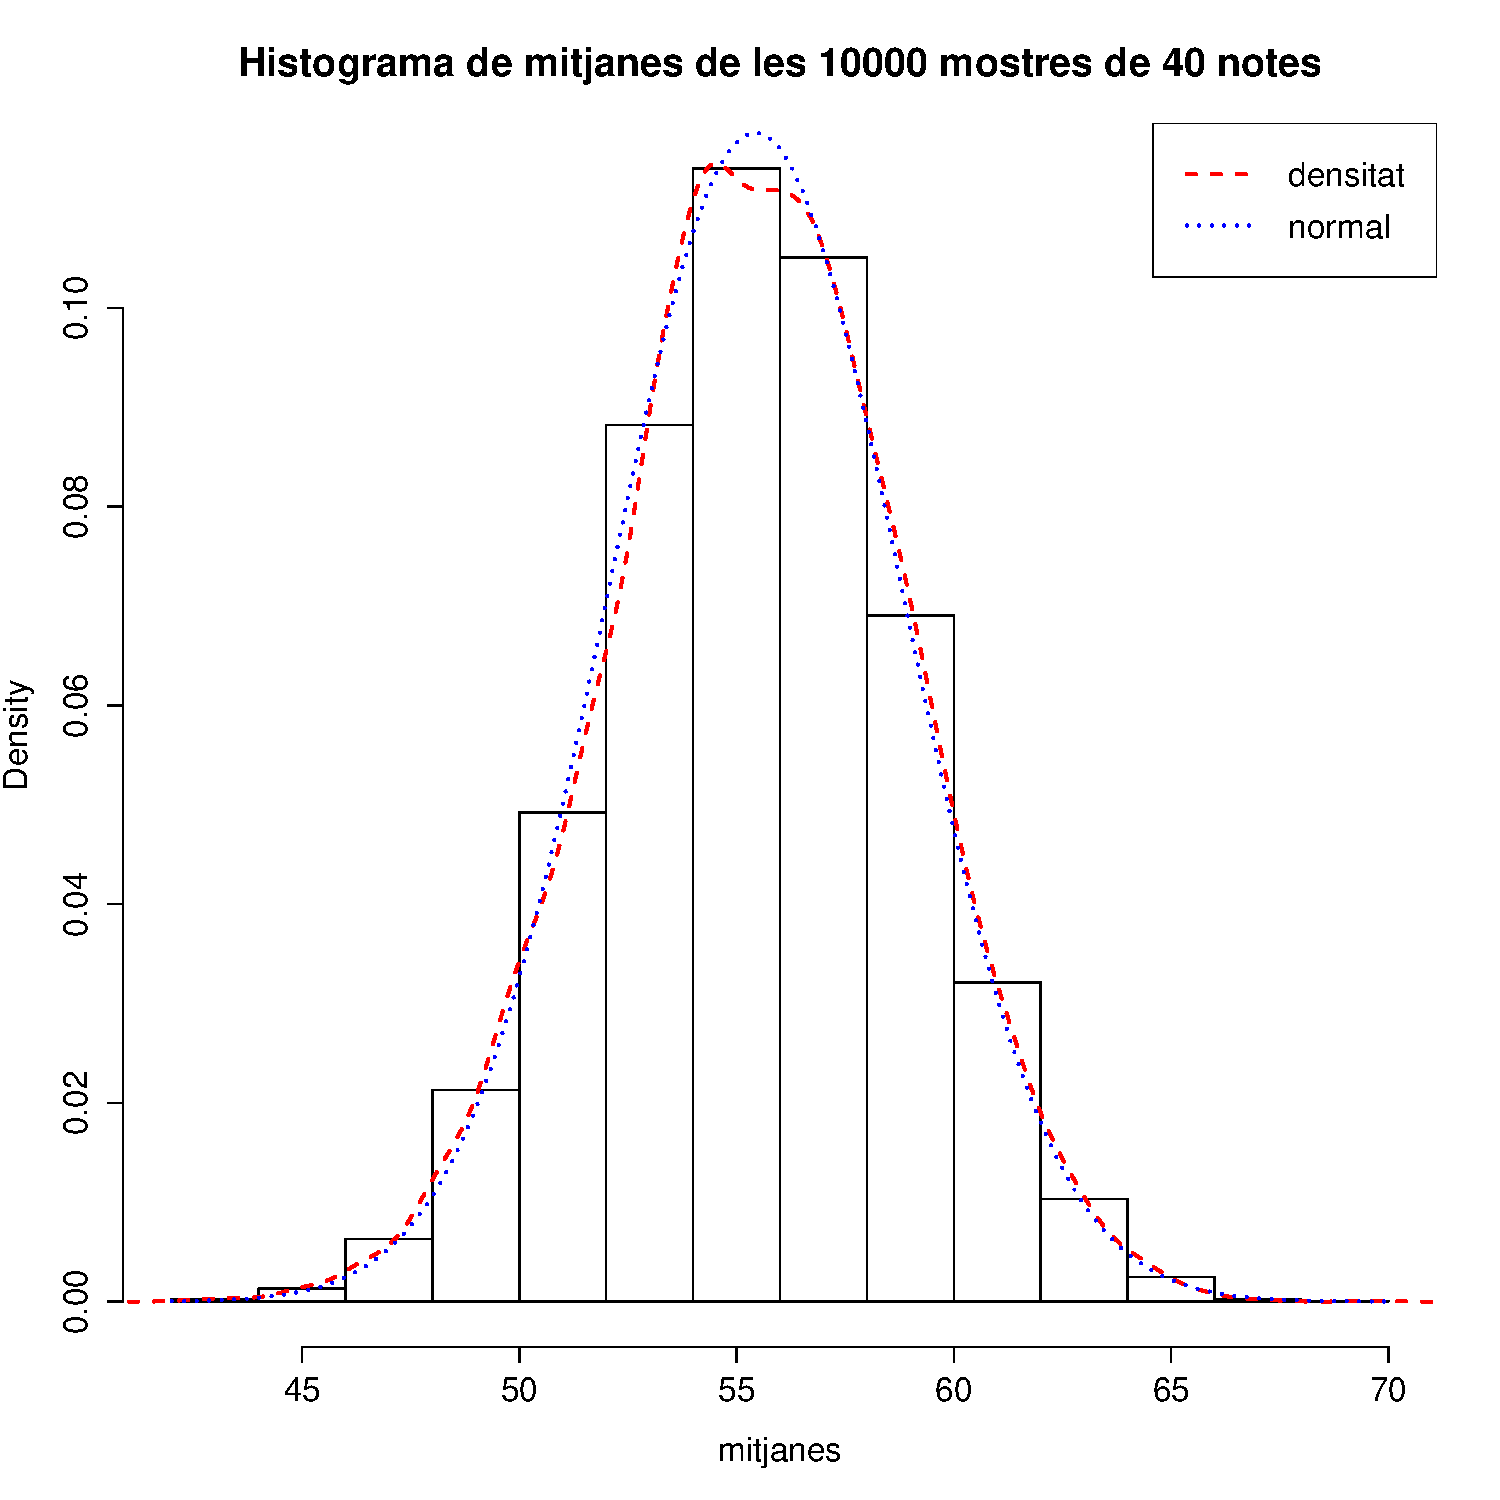
\includegraphics[width=0.8\linewidth]{hist-test}
\end{center}



\end{frame}




\begin{frame}
\frametitle{Exemple}
\vspace*{-2ex}

L'alçada d'una espècie de matolls té valor mitjà  $115$ cm, amb una desviació típica de $25$. Prenem una m.a.s.\ de $100$ matolls d'aquesta espècie.
\medskip

\blue{Quina és la probabilitat que la mitjana mostral de les alçades sigui $\leq 110$ cm?}
\medskip

$\displaystyle Z=\frac{\overline{X}-\mu_{X}}{\frac{\sigma_{X}}{\sqrt{n}}}=
\frac{\overline{X}-115}{2.5}$ és (\red{aproximadament}) $N(0,1)$
\medskip

$\begin{array}{rl}
P(\overline{X}\leq 110)  &\displaystyle= P\Big(Z\leq \frac{110-115}{2.5}\Big)= P(Z\leq -2)\\[2ex]
& \displaystyle=0.0228
\end{array}$


\end{frame}



\begin{frame}
\vspace*{-2ex}

\frametitle{Exemple}
L'alçada d'una espècie de matolls té valor mitjà  $115$ cm, amb una desviació típica de $25$. Prenem una m.a.s.\ de $100$ matolls d'aquesta espècie.
\medskip

\blue{Quina és la probabilitat que la mitjana mostral de les alçades estigui entre $113$ cm i $117$ cm?}
\pause\medskip

$\displaystyle Z=\frac{\overline{X}-115}{2.5}$ és $N(0,1)$
\medskip

$\begin{array}{l}
P(113\leq  \overline{X} \leq 117)  \displaystyle= P\Big(\frac{113-115}{2.5}\leq
  Z \leq \frac{117-115}{2.5}\Big)\\[2ex]
\quad \displaystyle =P(-0.8\leq
  Z \leq 0.8)= F_{Z}(0.8)-F_{Z}(-0.8)\\[1ex]
\quad \displaystyle = 2 F_{Z}(0.8) -1 = 2 \cdot 0.7881-1=0.5763
\end{array}$


\end{frame}








\begin{frame}
\frametitle{Mitjana mostral sense reposició}

Sigui $X_1,\ldots, X_n$ una m.a.\ \emph{sense reposició} de mida $n$ d'una v.a.\ $X$ d'esperança $\mu_X$ i desviació típica $\sigma_X$. 
\medskip

Si $n$ és  petit en relació a la mida $N$ de la població, tot funciona (per aproximació) com fins ara
\medskip

Si $n$ és gran en relació a $N$, aleshores
$$
E(\overline{X})=\mu_X,\quad \sigma_{\overline{X}}=\frac{\sigma_X}{\sqrt{n}}\cdot\red{\sqrt{\frac{N-n}{N-1}}}
$$
(\emph{factor de població finita})
\medskip

El T.C.L. ja no val tal qual en aquest darrer cas



\end{frame}

\subsection{Proporció mostral}
\begin{frame}
\frametitle{Proporció mostral}

Sigui $X$ una v.a.\ Bernoulli de paràmetre $p_X$ (1 èxit, 0 fracàs). Sigui $X_1,\ldots,X_n$ una m.a.s.\ de mida $n$ de $X$. 
\medskip

$S=\sum_{i=1}^n X_i$ és el nombre d'èxits observats. És $B(n,p)$.
\medskip

La \emph{proporció mostral} és 
$$
\widehat{p}_X=\frac{S}{n}
$$
i és un estimador de $p_X$
\medskip

Fixau-vos que $\widehat{p}_X$ és un cas particular de $\overline{X}$, per tant val tot el que hem dit fins ara per a mitjanes mostrals


\end{frame}


\begin{frame}
\frametitle{Proporció mostral}
$\widehat{p}_X=\dfrac{S}{n}$
\medskip

\begin{itemize}
\item $E(\widehat{p}_X)=p_X$
\medskip


\item $\displaystyle \sigma_{\widehat{p}_X}=\sqrt{\frac{p_X(1-p_X)}{n}}$, l'\emph{error estàndard} de la proporció mostral
\medskip

\item Si la mostra és sense reposició i $n$ és relativament gran,
$\displaystyle\sigma_{\widehat{p}_X}=\sqrt{\frac{p_X(1-p_X)}{n}}\cdot\red{\sqrt{\frac{N-n}{N-1}}}$
\end{itemize}

\end{frame}


\begin{frame}
\frametitle{Proporció mostral}
\vspace*{-2ex}

Pel T.C.L.:

\begin{block}{``Teorema''}
Si $n$ és gran (\emph{$n\geq 30$ o \underline{\textbf{40}}}) i la mostra és aleatòria simple, 
$$
\frac{\widehat{p}_X-p_X}{\sqrt{\frac{{p}_X(1-{p}_X)}{n}}}\approx N(0,1)
$$
\end{block}

\end{frame}


\begin{frame}
\frametitle{Exemple}
\vspace*{-2ex}

En una mostra aleatòria de 60 estudiants de la UIB del curs 2013-14, 37 varen ser dones. Estimau la fracció de dones entre els estudiants de la UIB
\pause\medskip

$$
\frac{37}{60}=0.6167
$$
\pause\vspace*{-2ex}

\begin{center}
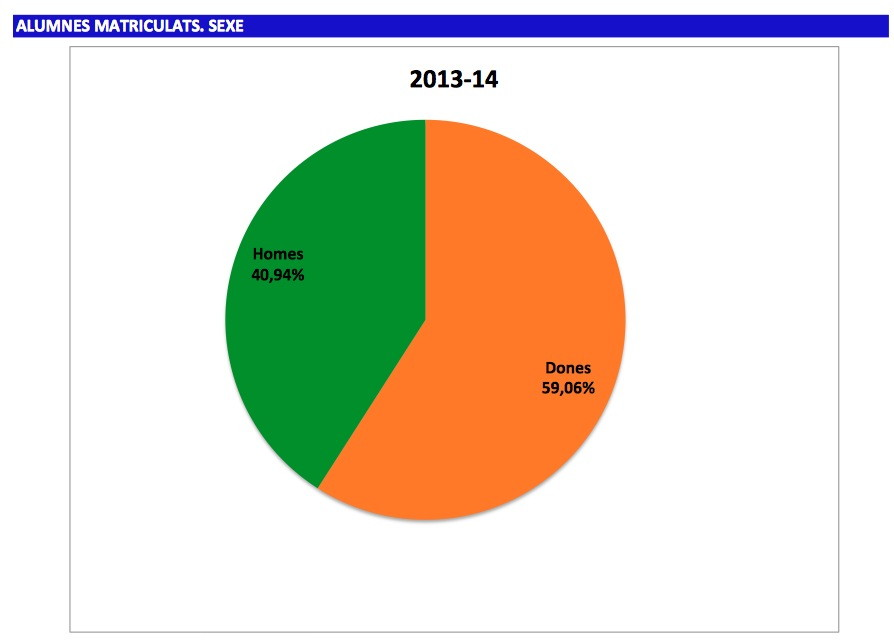
\includegraphics[width=0.7\linewidth]{sexeUIB}
\end{center}


\end{frame}


\begin{frame}
\frametitle{Exemple}
\vspace*{-2ex}

\blue{Un  59\% dels estudiants de la UIB són dones. Si prenem una m.a.s.\ de 60 estudiants, quina és la probabilitat que la proporció mostral de dones sigui superior al 61\%?}
\medskip \pause

$p_X=0.59$\\
$\widehat{p}_X\!\sim\! N\Bigg(0.59,\sqrt{\dfrac{0.59(1\!-\!0.59)}{60}}\Bigg)\!\!=\!N(0.59,0.0635)$
$$
Z=\frac{\widehat{p}_X-0.59}{0.0635}\sim N(0,1)
$$

$\begin{array}{l} 
\displaystyle P(\widehat{p}_X>0.61)= P\Bigg(\frac{\widehat{p}_X-0.59}{0.0635} > \frac{0.61-0.59}{0.0635}\Bigg)\\
  \quad\displaystyle  = P(Z > 0.315)=P(Z<-0.315)=0.3764
   \end{array}$
   \medskip
   
\end{frame}


\subsection{Variància mostral}

\begin{frame}
\frametitle{Variància mostral}

Sigui $X_1,\ldots, X_n$ una m.a.s.\ de mida $n$ d'una v.a.\ $X$ d'esperança $\mu_X$ i desviació típica $\sigma_X$
\medskip

La \emph{variància mostral} és
$$
\widetilde{S}_{X}^2=\frac{\sum_{i=1}^n (X_{i}-\overline{X})^2}{n-1}
$$
La \emph{desviació típica mostral} és 
$$
\widetilde{S}_{X}=+\sqrt{\widetilde{S}_{X}^2}
$$
A més, escriurem
$$
S^2_{X}=\frac{\sum_{i=1}^n (X_{i}-\overline{X})^2}{n}=\frac{(n-1)}{n}\widetilde{S}^2_{X}\quad\mbox{ i }\quad S_X=+\sqrt{S_X^2}
$$
\end{frame}


\begin{frame}
\frametitle{Variància mostral: Propietats}
\begin{itemize}
\item $\displaystyle S^2_X=\frac{\sum_{i=1}^n (X_{i}-\overline{X})^2}{n}=\left(\frac{\sum_{i=1}^n
X_{i}^2}{n}-\overline{X}^2\right)$\medskip

\item $\displaystyle \widetilde{S}_{X}^2=\frac{n}{n-1}\left(\frac{\sum_{i=1}^n
X_{i}^2}{n}-\overline{X}^2\right)$\medskip

\end{itemize}
\pause

\begin{teorema}
Si la v.a.\ $X$ és normal, aleshores $E(\widetilde{S}_{X}^2)=\sigma_{X}^2$ i 
la v.a.
$$
\frac{(n-1)\widetilde{S}_{X}^2}{\sigma_{X}^2}
$$
té distribució $\chi_{n-1}^2$
\end{teorema}
\end{frame}


\begin{frame}
\frametitle{La distribució $\chi_n^2$}

La distribució $\chi_n^2$ ($\chi$: en català, \emph{khi}; en castellà, \emph{ji}; en anglès, \emph{chi}), on $n$ són els \emph{graus de llibertat}:
\begin{itemize}
\item És la de 
$$
X=Z_{1}^{2}+Z_{2}^{2}+\cdots +Z_{n}^{2}
$$ 
on  $Z_{1},Z_{2},\ldots, Z_{n}$ son v.a.\  independents  $N(0,1)$
\medskip

\item Té densitat
$$
f_{\chi_n^2}(x)={\frac{1}{2^{n/2} \Gamma (n/2)}} x^{(n/2)-1} e^{-x/2}\quad\mbox{ si $x\geq 0$}
$$
on $\Gamma(x)=\int_{0}^{\infty} t^{x-1}e^{-t}\, dt$ si $x> 0$

\end{itemize}
\end{frame}


\begin{frame}
\frametitle{La distribució $\chi_n^2$}

\begin{itemize}
\item La distribució està tabulada (\emph{Teniu les taules a Campus Extens}), i amb R és \texttt{chisq}
\bigskip

\item Si $X_{\chi_n^2}$ és una v.a.\ amb distribució  $\chi_n^2$,
$$E(X_{\chi_n^2})=n,\quad Var(X_{\chi_n^2})=2 n$$
\medskip

\item ${\chi_n^2}$ s'aproxima a una distribució normal $N(n,\sqrt{2n})$ per a $n$ gran
($n>40$ o $50$) 
\end{itemize}

\end{frame}

\begin{frame}
\frametitle{La distribució $\chi_n^2$}
\vspace*{-1cm}

\begin{center}
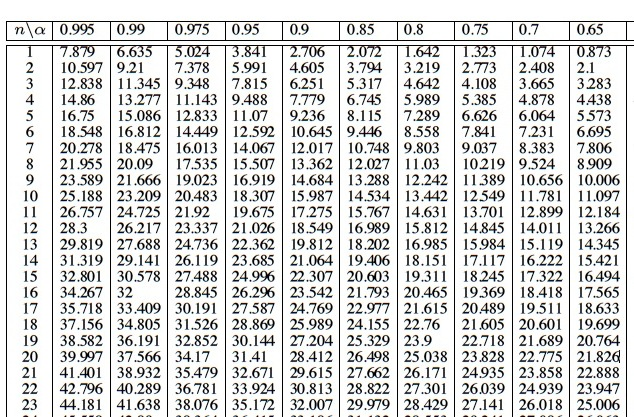
\includegraphics[width=\linewidth]{taulachi.jpg}
\end{center}

$F_{\chi_{10}^2}(25.188)=0.995$,\  $F_{\chi_{20}^2}(26.5)\approx 0.85$\quad  \blue{Feu el test!}

\end{frame}


\begin{frame}
\frametitle{La distribució $\chi_n^2$}
\vspace*{-1cm}

\begin{center}
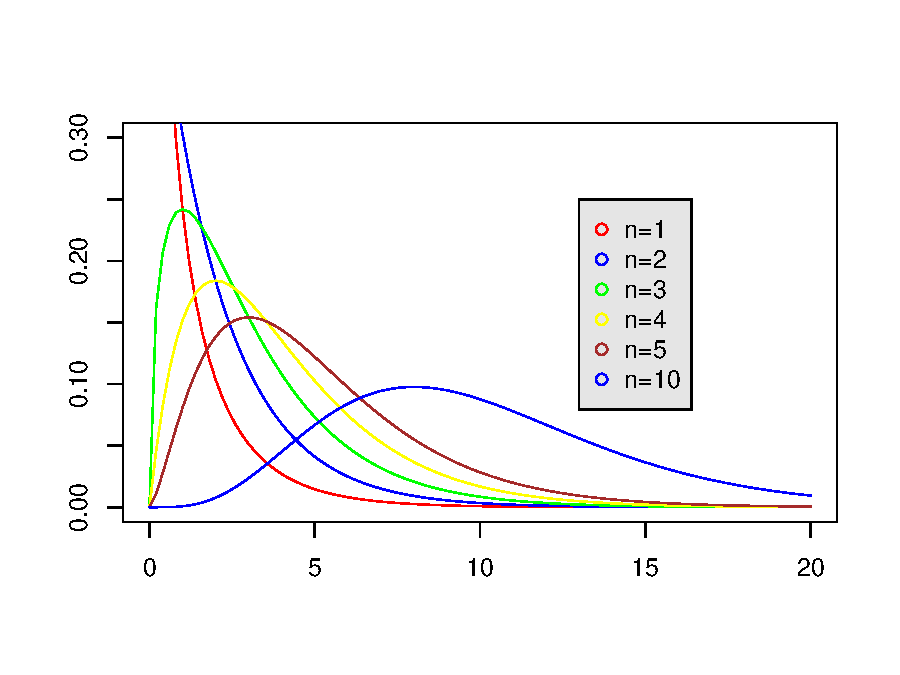
\includegraphics[width=\linewidth]{./dibujos-001}

Funció  de densitat de $\chi^2_n$ per a alguns $n$
\end{center}
\end{frame}

\begin{frame}
\frametitle{Exemple}
\vspace*{-2ex}

L'augment diari del pes d'un pollastre d'una granja segueix una
distribució normal amb desviació típica $1.7$. Es pren una
mostra de 12 pollastres. Suposam que aquesta mostra és petita respecte del total de la població de la granja.
\medskip

\blue{Probabilitat que la desviació típica mostral
sigui $\leq 2.5$?}
\medskip

Sigui $X$= l'augment diari del pes d'un pollastre. Sabem que $\sigma_{X}^2=(1.7)^2=2.89$. Com que $X$ és normal
 i $n=12$, tenim que
$$
\frac{11\cdot \widetilde{S}_{X}^2}{2.89}=\frac{(n-1)\widetilde{S}_{X}^2}{\sigma_{X}^2}\sim \chi^2_{11}
$$

        
\end{frame}


\begin{frame}
\frametitle{Exemple}
\vspace*{-2ex}

L'augment diari del pes d'un pollastre d'una granja segueix una
distribució normal amb desviació típica $1.7$. Es pren una
mostra de 12 pollastres. Suposam que aquesta mostra és petita respecte del total de la població de la granja.
\medskip

\blue{Probabilitat que la desviació típica mostral
sigui $\leq 2.5$?}
\medskip

$\dfrac{11\widetilde{S}_{X}^2}{2.89}\sim \chi^2_{11}$
\medskip

$\begin{array}{l}
\displaystyle P(\widetilde{S}_{X}<2.5)= P\left(\widetilde{S}_{X}^2<2.5^2\right)\\
\quad \displaystyle =P\left(\frac{11\cdot \widetilde{S}_{X}^2}{2.89}<\frac{11
\cdot 2.5^2}{2.89}\right)= P(\chi_{11}^2<23.79)\\
\only<2>{\quad\displaystyle=\mbox{\texttt{pchisq(23.7889,11)}}=0.986}
\only<3>{\quad \displaystyle \approx P(\chi_{11}^2<24.725)=0.99}
\end{array}$
        
\end{frame}


\subsection{Propietats dels estimadors}


\begin{frame}
\frametitle{Estimadors no esbiaixats}

Quan un estimador és bo?
\medskip

Un estimador puntual $\widehat{\theta}$ d'un paràmetre poblacional
$\theta$ és  \emph{no esbiaixat} quan el seu valor esperat és precisament el valor del paràmetre:
$$
E(\widehat{\theta})=\theta
$$ 
Es diu aleshores que l'estimació puntual és \emph{no esbiaixada}.
\medskip

El  \emph{biaix} de $\widehat{\theta}$ és $E(\widehat{\theta})-\theta$

\end{frame}


\begin{frame}
\frametitle{Estimadors no esbiaixats}


\blue{Exemples}

\begin{itemize}
\item $E(\overline{X})=\mu_X$: $\overline{X}$ és estimador no esbiaixat de $\mu_X$
\medskip

\item $E(\widehat{p}_X)=p_X$: $\widehat{p}_X$ és estimador no esbiaixat de $p_X$
\medskip

\item $E(\widetilde{S}_{X}^2)=\sigma_X^2$ si $X$ és normal: $\widetilde{S}_{X}^2$ és estimador no esbiaixat de $\sigma_X^2$ quan $X$ és normal
\medskip

\item $E({S}_{X}^2)=\dfrac{n-1}{n}\sigma_X^2$ si $X$ és normal; per tant
\emph{${S}_{X}^2$ és esbiaixat}, amb biaix
$$
E({S}_{X}^2)-\sigma_X^2=\dfrac{n-1}{n}\sigma_X^2-\sigma_X^2=-\dfrac{\sigma_X^2}{n}\ \tendeix\ 0
$$

\end{itemize}

\end{frame}


\begin{frame}
\frametitle{Estimadors eficients}

Quan un estimador és \emph{millor}?
\medskip

Quan és no esbiaixat i té poca variabilitat (així és més probable que aplicat a una m.a.s.\ doni prop del valor esperat)
\medskip

\emph{Error estàndard d'un estimador $\widehat{\theta}$}: la seva desviació típica
$$\sigma_{\widehat{\theta}}=\sqrt{Var(\widehat{\theta})}$$
\medskip

\end{frame}


\begin{frame}
\frametitle{Estimadors eficients}

Donats dos estimadors $\widehat{\theta}_1$, $\widehat{\theta}_2$ no esbiaixats (o amb biaix $\tendeix 0$) del mateix paràmetre $\theta$, direm que 
\begin{center}
$\widehat{\theta}_1$ és \emph{més eficient} que $\widehat{\theta}_2$
\end{center}
 quan $$\sigma_{\widehat{\theta}_1}< \sigma_{\widehat{\theta}_2},$$  és a dir, quan $$Var(\widehat{\theta}_1)< Var(\widehat{\theta}_2)$$


\end{frame}


\begin{frame}
\frametitle{Estimadors eficients}

\blue{Exemple}: Sigui $X$ una v.a.\ amb mitjana $\mu_X$ i desviació típica $\sigma_X$
\medskip

Considerem la mediana $Me=Q_{0.5}$ de la realització d'una m.a.s.\ de $X$ com a estimador puntual de $\mu_X$
\medskip

Si $X$ és normal, 
$$
\begin{array}{l}
E(Me)=\mu_X,\\
\displaystyle  Var(Me)\approx \frac{\pi}{2}
     \frac{\sigma_{X}^2}{n}\approx \frac{1.57 \sigma_{X}^2}{n}=1.57Var(\overline{X})
\end{array}
$$
Per tant, $Me$ és un estimador no esbiaixat de   $\mu_X$, però menys eficient que $\overline{X}$



\end{frame}


\begin{frame}
\frametitle{Estimadors  eficients}

\begin{itemize}
\item Si la població és normal, la mitjana mostral és l'estimador
no esbiaixat més eficient de la mitjana poblacional
\medskip

\item Si la població és Bernoulli, la proporció mostral és l'estimador
no esbiaixat més eficient de la proporció poblacional
\medskip

\item Si la població és normal, la variància mostral és l'estimador
no esbiaixat  més eficient de la variància poblacional
 \end{itemize}




\end{frame}


\begin{frame}
\frametitle{Estimadors  eficients}

Hem dit que si la població és normal, la variància mostral és l'estimador
no esbiaixat  més eficient de la variància poblacional
\medskip

L'estimador ``variància''
$$
S_X^2=\frac{(n-1)}{n} \widetilde{S}_X^2
$$   
encara és més eficient, però  té biaix $\tendeix 0$
\medskip

Si $n$ és petit ($\leq 30$ o 40), és millor fer servir la variància mostral $\widetilde{S}_X^2$ per estimar la variància, ja que el biaix influeix, però si $n$ és gran, el biaix ja no és tan important i es pot fer servir $S_X^2$


\end{frame}



\begin{frame}
\frametitle{Exemple: Estimació de poblacions}

Tenim una població numerada $1,2,\ldots,N$\medskip

En prenem una m.a.s. $x_1,\ldots,x_n$; sigui
$m=\max(x_1,\ldots,x_n)$
\medskip

\begin{block}{Teorema}
L'estimador no esbiaixat més eficient de $N$ és
$$
\widehat{N}=m+\frac{m-n}{n}
$$
\end{block}
\bigskip


Un problema de rellevància històrica:

{\scriptsize \url{http://en.wikipedia.org/wiki/German_tank_problem}}

\end{frame}



\begin{frame}[fragile]
\frametitle{Exemple: Estimació de poblacions}
\vspace*{-2ex}

\blue{Exemple:}
Assegut en un bar del Passeig Marítim he apuntat les llicències dels 40 primers taxis que he vist:
\vspace*{-1ex}

{\footnotesize
\begin{verbatim}
> taxis=c(1217,600,883,1026,150,715,297,137,508,134,
  38,961,538,1154,314,1121,823,158,940,99,977,286,
  1006,1207,264,1183,1120,498,606,566,1239,860,114,
  701,381,836,561,494,858,187)
\end{verbatim}
}
\vspace*{-1ex}

Suposaré que formen una m.a.s. dels taxis de Palma. Aleshores, estim que el nombre de taxis de Palma 
és
\vspace*{-1ex}

{\footnotesize
\begin{verbatim}
> N=max(taxis)+(max(taxis)-length(taxis))/length(taxis)
> N
[1] 1268.975
\end{verbatim}
}
\vspace*{-1ex}

En realitat, n'hi ha 1246 
\medskip

{\scriptsize \url{http://www.caib.es/eboibfront/es/2014/10195/551436/departamento-de-movilidad-seccion-de-transportes-r}

}


\end{frame}

\begin{frame}
\frametitle{Estimadors màxim versemblants}

\blue{Com trobam bons estimadors?}
\medskip

Sigui $X$ una v.a.\ \emph{discreta} amb densitat 
$$
f_X(x;\lambda)
$$
que depèn d'un
paràmetre desconegut $\lambda$
\medskip

Sigui $X_{1},\ldots X_{n}$ una m.a.s.\ de $X$, i sigui $x_1,x_2,\ldots,x_n$ una realització d'aquesta mostra
\medskip


La \emph{funció de versemblança} de la mostra és la probabilitat condicionada següent:
$$
\begin{array}{rl}
\red{L(\lambda|x_1,x_2,\ldots,x_n)} & := P(x_1,x_2,\ldots,x_n|\lambda)\\&=P(X_1=x_1)\cdots P(X_n=x_n)\\
& = f_X(x_1;\lambda)\cdots f_X(x_n;\lambda)
\end{array}
$$

\end{frame}

\begin{frame}
\frametitle{Estimadors màxim versemblants}

Donada la funció de versemblança $L(\lambda|x_1,\ldots,x_n)$ de la mostra, indicarem per 
$$
\red{\hat{\lambda}(x_1,\ldots,x_n)}
$$ 
el valor del paràmetre $\lambda$ on s'aconsegueix el màxim
de $L(\lambda|x_1,\ldots,x_n)$. Serà una funció de $x_1,\ldots,x_n$.
\medskip


\begin{defin}
\begin{small}
Un estimador $\hat{\lambda}$ d'un paràmetre $\lambda$ és \emph{màxim versemblant} (\emph{MV}, en anglès \emph{EM}) quan, per a cada m.a.s, la probabilitat d'observar-la és màxima quan el paràmetre pren el valor de l'estimador aplicat a la mostra, és a dir, quan la funció de versemblança
$$L(\lambda|x_1,x_2,\ldots,x_n)= P(x_1,x_2,\ldots,x_n|\lambda)$$
 assoleix el seu màxim.
 \end{small}
\end{defin}
\end{frame}

\begin{frame}
\frametitle{Estimadors màxim versemblants}

\blue{Exemple}: Suposem que tenim una v.a. Bernoulli $X$ de probabilitat d'èxit $p$ desconeguda\medskip

Per a cada m.a.s. $x_1,\ldots,x_n$ de $X$, siguin \red{$\widehat{p}_x$} la seva proporció mostral i  \red{$P(x_1,\ldots,x_n\mid p)$} la probabilitat d'obtenir-la quan el paràmetre pren el valor $p$

\begin{block}{Teorema}
El valor de $p$ per al qual $P(x_1,\ldots,x_n\mid p)$ és màxim és $\widehat{p}_x$.
\end{block}

La proporció mostral és un estimador MV de $p$. Vegem-ho. 

\end{frame}


\begin{frame}
\frametitle{Estimadors màxim versemblants}

\vspace{1cm}

\begin{obs}
En general, com que $\ln$ és creixent, en lloc de maximitzar $L(\lambda|x_1,\ldots,x_n)$, maximitzam
$$
\ln(L(\lambda|x_1,\ldots,x_n))
$$
que sol ser més fàcil (productes $\to$ sumes).
\end{obs}
\end{frame}


\begin{frame}
\frametitle{Estimadors màxim versemblants}
Sigui $X_{1},\ldots X_{n}$ una m.a.s.\ d'una v.a.\ Bernoulli $X$ de paràmetre $p$ (desconegut). Posem $q=1-p$
$$
\begin{array}{c}
f_X(1;p)=P(X=1)=p,\quad 
f_X(0;p)=P(X=0)=q
\end{array}
$$
és a dir, per $x\in\{0,1\}$, resulta que 
$$f_X(x;p)=P(X=x)=p^{x} q^{1-x}.$$

La funció de versemblança és:
$$
\begin{array}{l}
L(p|x_1,\ldots,x_n) = f_{X}(x_1;p)\cdots f_{X}(x_n;p)\\[1ex]
\quad =
p^{x_{1}}q^{1-x_{1}} \cdots  p^{x_{n}}q^{1-x_{n}}
\\[1ex]
\quad = p^{\sum_{i=1}^n x_{i}} q^{\sum_{i=1}^n (1-x_{i})}= p^{\sum_{i=1}^n x_{i}} q^{n-\sum_{i=1}^n x_{i}}\\[1ex]
\quad =p^{\sum_{i=1}^n x_{i}} (1-p)^{n-\sum_{i=1}^n x_{i}}
\end{array}
$$
\end{frame}

\begin{frame}
\frametitle{Exemple}
La funció de versemblança és
$$
\begin{array}{rl}
L(p|x_1,\ldots,x_n) & =p^{\sum_{i=1}^n x_{i}} (1-p)^{n-\sum_{i=1}^n x_{i}}\\
& =p^{n\overline{x}}(1-p)^{n-n\overline{x}}
\end{array}
$$
on $\overline{x}=\dfrac{\sum_{i=1}^n x_{i}}{n}$
\medskip


Volem trobar el valor de $p$ on s'assoleix el màxim d'aquesta funció (on $\overline{x}$ és un paràmetre: la variable és $p$)
\medskip

Maximitzarem el seu logaritme:
$$
\begin{array}{l}
\ln(L(p|x_1,\ldots,x_n))\\
\qquad \displaystyle=n\overline{x}\ln(p)+n(1-\overline{x})\ln(1-p)
\end{array}
$$
\end{frame}

\begin{frame}
\frametitle{Exemple}
Derivem respecte de $p$:
$$
\begin{array}{l}
\ln(L(p|x_1,\ldots,x_n))'\\
\qquad \displaystyle=n\overline{x}\frac{1}{p}-n(1-\overline{x})\frac{1}{1-p}\\
\qquad \displaystyle=\frac{1}{p(1-p)}\Big((1-p)n\overline{x}-pn(1-\overline{x})\Big)\\
\qquad \displaystyle=\frac{1}{p(1-p)}(n\overline{x} -pn)=\frac{n}{p(1-p)}(\overline{x} -p)\\
\end{array}
$$
Estudiem el signe:
$$
\begin{array}{rl}
\ln(L(p|x_1,\ldots,x_n))'\geq 0 &\displaystyle \Leftrightarrow \overline{x} -p\geq 0\\ &\displaystyle \Leftrightarrow
p\leq\overline{x}
\end{array}
$$
\end{frame}

\begin{frame}
\frametitle{Exemple}
Per tant
$$
\ln(L(p|x_1,\ldots,x_n))\left\{
\begin{array}{l}
\mbox{ creixent fins $\overline{x}$}\\
\mbox{ decreixent a partir de $\overline{x}$}\\
\mbox{ \red{té un màxim a $\overline{x}$}}
\end{array}\right.
$$

\vspace{1cm}

I el resultat queda demostrat. $L(\widehat{p}_X|x_1,\ldots,x_n)\geq L(p|x_1,\ldots,x_n)$ per a qualsevol  $p$
\end{frame}

\begin{frame}
\frametitle{Alguns estimadors MV}
\vspace*{-1ex}

\begin{itemize}
\item $\widehat{p}_x$ és l'estimador MV del paràmetre $p$ d'una v.a. Bernoulli
\medskip

\item $\overline{X}$  és l'estimador MV del paràmetre $\lambda$ d'una v.a. Poisson
\medskip

\item $\overline{X}$  és l'estimador MV del paràmetre $\mu$ d'una v.a. normal
\medskip

\item $S_X^2$ (\red{\underline{no} $\widetilde{S}_X^2$}) és l'estimador MV del paràmetre $\sigma^2$ d'una v.a. normal
\medskip

\item El màxim (\red{\underline{no}  $\widehat{N}$}) és l'estimador MV de la $N$ al problema dels taxis

\end{itemize}

\end{frame}


\begin{frame}
\frametitle{Exemple: $\lambda$ per a una Poisson}

\vspace{1cm}

\begin{block}{}
Sigui $X$ una característica d'una població que segueix una llei $Po(\lambda)$, amb $\lambda>0$ desconegut. Prenem una mostra aleatòria simple $X_1,\ldots,X_n$ d'aquesta població i obtenim els resultats $x_1,\ldots,x_n$. 
\medskip

Trobau l'estimador màxim versemblant de $\lambda$ per a $x_1,\ldots,x_n$.
\end{block}
\end{frame}

\begin{frame}
\frametitle{Exemple: $\lambda$ per a una Poisson}

Primer hem de trobar 
la funció de versemblança $L(\lambda\mid x_1,\ldots,x_k)$.
\medskip

Si $X\sim Pois(\lambda)$, sabem que $P(X=x_i)=e^{-\lambda}\cdot \dfrac{\lambda^{x_i}}{x_i!}$ i per tant
$$
\begin{array}{l}
L(\lambda\mid x_1,\ldots,x_k)  =\displaystyle P(X=x_1)\cdot P(X=x_2)\cdots P(X=x_n)\\[1ex] \quad =\pause\displaystyle 
\Big(e^{-\lambda}\cdot \frac{\lambda^{x_1}}{x_1!}\Big)\cdot \Big(e^{-\lambda}\cdot \frac{\lambda^{x_2}}{x_2!}\Big)\cdots \Big(e^{-\lambda}\cdot \frac{\lambda^{x_n}}{x_n!}\Big)\\[1ex] \quad =\displaystyle e^{-n\lambda}\cdot \frac{\lambda^{x_1+\cdots+x_n}}{x_1!\cdots x_n!}=e^{-n\lambda}\cdot \frac{\lambda^{n\overline{x}}}{x_1!\cdots x_n!}

\end{array}
$$
\end{frame}

\begin{frame}
\frametitle{Exemple: $\lambda$ per a una Poisson}

Ara volem trobar el valor de $\lambda$ que maximitza 
$$
f(\lambda)\!:=\!\ln(L(\lambda\mid x_1,\ldots,x_k))\!=\!-n\lambda+n\overline{x}\ln(\lambda)-\ln(x_1!\cdots x_n!)
$$
\pause
Derivem respecte de $\lambda$
$$
f'(\lambda)=-n+n\overline{x}\cdot \frac{1}{\lambda}=
\frac{n(\overline{x}-\lambda)}{\lambda}
$$
Com que $n,\lambda>0$, tenim que 
$$
f'(\lambda)\left\{\begin{array}{ll}
>0 &\mbox{ si $\lambda<\overline{x}$}\\[1ex]
<0 &\mbox{ si $\lambda>\overline{x}$}\\[1ex]
=0 &\mbox{ si $\lambda=\overline{x}$}
\end{array}\right.
$$
\end{frame}

\begin{frame}
\frametitle{Exemple: $\lambda$ per a una Poisson}
Per tant,
$$
\ln(L(\lambda\mid x_1,\ldots,x_k))\left\{\begin{array}{l}
\mbox{és creixent a $]0,\overline{x}[$}\\[1ex]
\mbox{és decreixent a $]\overline{x},\infty[$}\\[1ex]
\mbox{té el màxim a $\lambda=\overline{x}$}
\end{array}\right.
$$
\begin{block}{Teorema}
L'estimador màxim versemblant per a $\lambda$ és la mitjana  $\overline{x}$.
\end{block}
\end{frame}

\begin{frame}
\frametitle{Exemple: Marca-recaptura}

En una població hi ha $N$ individus, en capturam $K$, els marcam i els tornam a amollar.  Ara en tornam a capturar $n$, dels quals $k$ estan marcats. A partir d'aquestes dades, volem estimar $N$.
\bigskip

Suposam que $N$ i $K$ no han canviat de la primera a la segona captura
\bigskip

$X=$``Un individu estigui marcat'' és $Be(p)$ amb $p=\dfrac{K}{N}$
\bigskip

$X_1,\ldots,X_n$ la mostra capturada en segon lloc: $\widehat{p}_X=\dfrac{k}{n}$

\end{frame}


\begin{frame}
\frametitle{Exemple: Marca-recaptura}

$\widehat{p}_X$ és estimador màxim versemblant de $p$: Estimam que
$$
\dfrac{K}{N}=\dfrac{k}{n}\Rightarrow N=\frac{n\cdot K}{k}
$$

Per tant, l'estimador
$$
\red{\widehat{N}=\frac{n\cdot K}{k}}
$$
 maximitza la probabilitat de l'observació ``$k$ marcats de $n$ capturats''. És l'\emph{estimador màxim versemblant} de $N$.

\end{frame}

\begin{frame}
\frametitle{Exemple: Marca-recaptura}

Suposem que hem marcat 15 peixos del llac, i que en una captura de 10 peixos, n'hi ha 4 de marcats. Quants peixos estimau que conté el llac?
\medskip

$$
\widehat{N}=\frac{15\cdot 10}{4}=37.5
$$
Per tant, estimam que hi haurà entre 37 i 38 peixos al llac

\end{frame}


\begin{frame}[fragile]
\frametitle{Exemple: Marca-recaptura}
\vspace*{-0.8cm}

$$
P(\mbox{$k$ marcats de $n$ capturats})=\dfrac{\binom{K}{k}\cdot \binom{N-K}{n-k}}{\binom{N}{n}}
$$

\begin{verbatim}
> N=15:100
> p=choose(15,4)*choose(N-15,6)/choose(N,10)
> plot(N,p,type="h",xaxp=c(15,100,17))
\end{verbatim}
\vspace*{-4ex}

\begin{center}
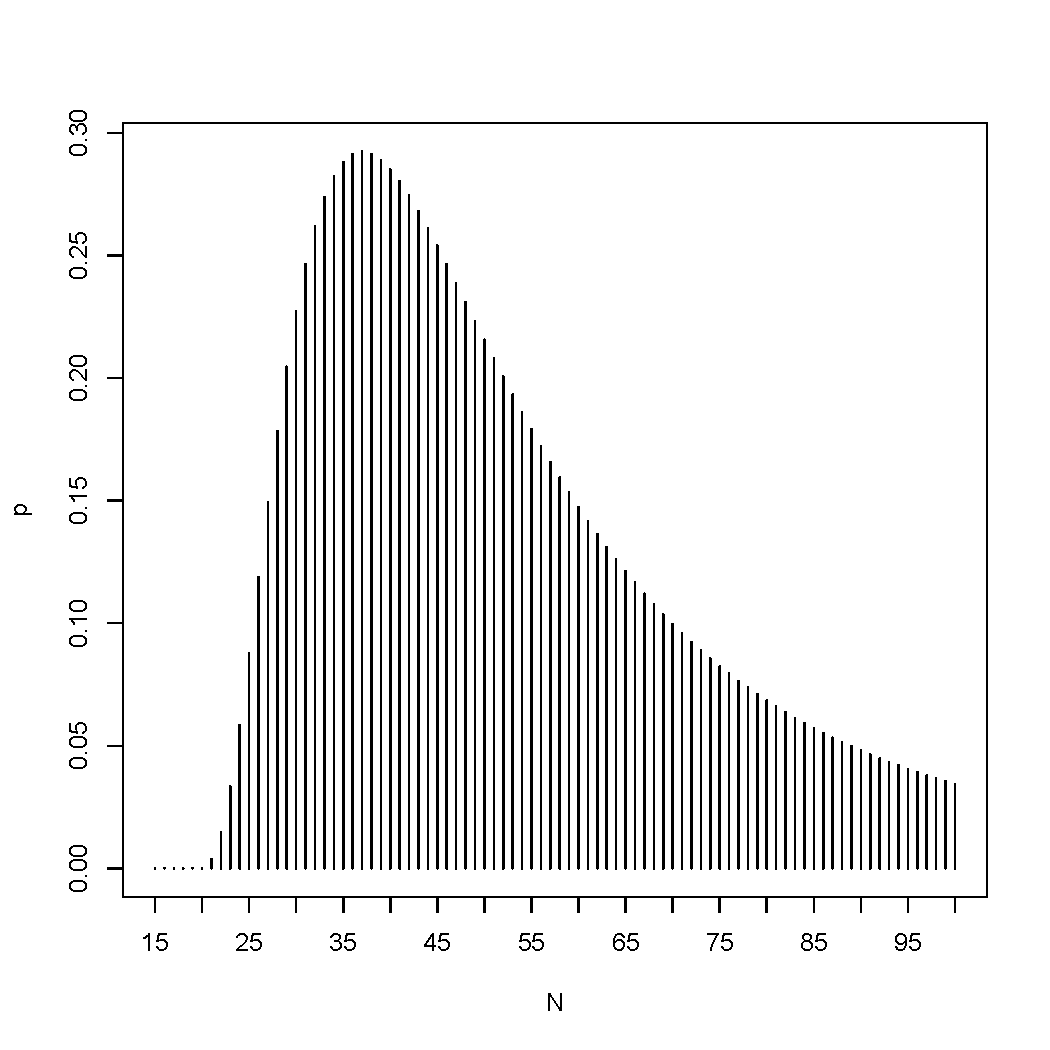
\includegraphics[width=0.65\linewidth]{marca.pdf}
\end{center}


\end{frame}


\begin{frame}
\frametitle{Exemple: Marca-recaptura}

L'estimador
$$
\widehat{N}=\frac{n\cdot K}{k}
$$
és esbiaixat, amb biaix $\tendeix 0$
\bigskip

L'\emph{estimador de Chapman}
$$
\widehat{N}=\frac{(n+1)\cdot (K+1)}{k+1}-1
$$
és menys esbiaixat per a mostres petites, i no esbiaixat si $K+n\geq N$ (però no màxim versemblant)
\end{frame}


\end{document}



